\documentclass[12pt]{article}
\usepackage[utf8]{inputenc}
\usepackage{setspace}
\usepackage[left=1in, right=1in, top=1in, bottom=1in]{geometry}
\usepackage{amsmath,amsfonts,amssymb}
\usepackage{graphicx}
\usepackage{hyperref}


% MLA Style Title Page
\title{The Interplay of the Fibonacci Sequence and Golden Ratio in Mobile Ad Hoc Networks}
\author{Marty Martin}
\date{\today}

\begin{document}

\maketitle
\thispagestyle{empty}
\clearpage

\setcounter{page}{1}
\doublespacing % Sets 1.5 line spacing

% Introduction Section
The Fibonacci sequence is one of the most fascinating mathematical concepts, with its simple recursive definition leading to a wealth of intriguing properties and applications across diverse fields. This sequence, in which each number is the sum of the two preceding ones, produces the series 1, 1, 2, 3, 5, 8, 13, 21, and so on into infinity. Closely related to the Fibonacci numbers is the golden ratio, an irrational number approximately equal to 1.618 that possesses many alluring mathematical properties. A scientific paper "Fibonacci sequence based multipath load balancing approach for mobile ad hoc networks," Tashtoush et al. address the pressing issues of congestion and packet loss in MANETs. These networks, devoid of centralized infrastructure, consist of mobile nodes that independently self-organize, dynamically adapting to the ever-changing network topology. As nodes move, the routes between them often break, and the limited bandwidth is easily overwhelmed, resulting in significant packet loss. This section will delve into the innovative solutions proposed by Tashtoush et al., illustrating how they harness the Fibonacci sequence to enhance load balancing in MANETs, thereby mitigating these challenges and demonstrating a practical application of mathematical principles in addressing real-world problems.

% Summary of the Scientific Paper Section
In their paper ``Fibonacci sequence based multipath load balancing approach for mobile ad hoc networks,'' Tashtoush et al. tackle the problem of congestion and dropped packets in MANETs. A MANET is a decentralized network of mobile wireless nodes that can dynamically self-organize and forward traffic without relying on fixed infrastructure. With nodes constantly moving around, the network topology rapidly changes, routes between nodes frequently break, and the limited bandwidth gets congested - leading to many dropped packets.

To improve the packet delivery ratio, the authors propose a novel load balancing scheme called the Fibonacci Multipath Load Balancing (FMLB) protocol. The key idea is to discover multiple paths between the source and destination nodes and distribute the transmitted packets across these paths using the Fibonacci sequence. Specifically, the available paths are sorted in increasing order of length (number of hops). Each path is then assigned a Fibonacci number based on its position in this sorted list - the shortest path gets the largest Fibonacci number and so on. Finally, packets are allocated to the paths proportional to their assigned Fibonacci weights.

\begin{figure}[ht]
  \centering
  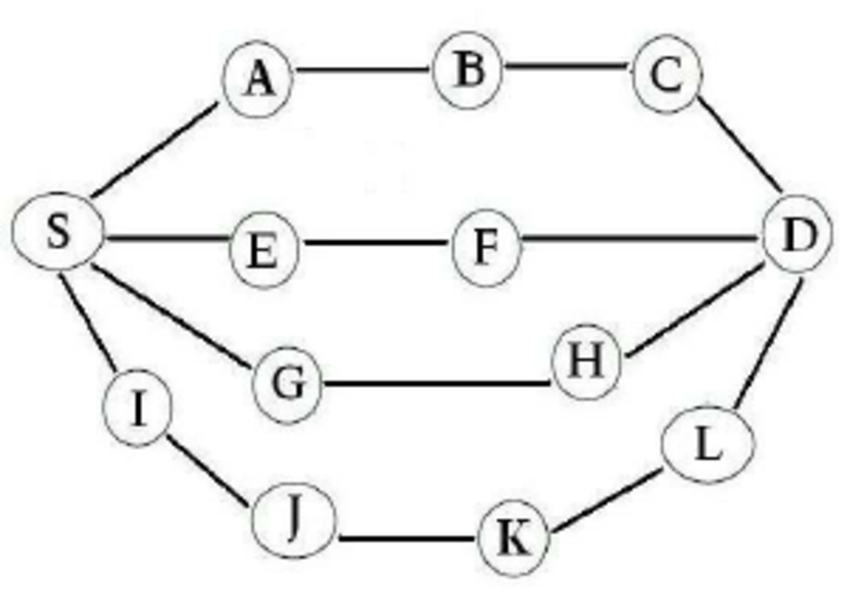
\includegraphics[width=0.3\textwidth]{./images/Multiple-paths-between-source-and-destination.png}
  \caption{Multiple paths between source and destination.}
  \label{fig:multiple_paths_map}
  \end{figure}

For example, if there are 5 paths with 2, 3, 4, 5, and 6 hops respectively, they would be assigned the Fibonacci numbers $5, 3, 2, 1, 1$. The fraction of packets allocated to each path would then be $\frac{5}{12}, \frac{3}{12}, \frac{2}{12}, \frac{1}{12}, \frac{1}{12}$. In this way, the shorter paths are utilized more heavily than the longer paths, but the longer paths still serve to alleviate congestion on the shorter ones. Through analysis and simulations, the authors show that this Fibonacci-based load balancing approach achieves significant gains in packet delivery compared to standard single-path routing as well as other multi-path schemes.

% Connection to Fibonacci Numbers Section
It is quite amazing that the humble Fibonacci sequence, which starts out as $1, 1, 2, 3, 5$, would be useful for routing packets in a wireless network! The authors' choice of using Fibonacci numbers for path weights has some interesting mathematical properties and consequences worth exploring.

The Fibonacci numbers are defined by the recurrence relation:
\begin{equation}
F_0 = 0, \quad F_1 = 1, \quad F_n = F_{n-1} + F_{n-2} \text{ for } n > 1.
\end{equation}

In the FMLB protocol, the paths are assigned weights $F_k, F_{k-1}, \ldots, F_2, F_1$ where $k$ is the number of available paths. This means the ratios of the path weights, and thus the fraction of packets allocated, are approximately in proportion to the golden ratio. To see this, note that for large $n$, the ratio of successive Fibonacci numbers converges to the golden ratio $\varphi$:

\begin{equation}
\lim_{n \to \infty} \frac{F_n}{F_{n-1}} = \varphi \approx 1.618.
\end{equation}

In figure 1 the example with 5 paths, the ratios of the packets allocated is roughly calculated as follows and can be directly compared with the findings in Tashtoush et al.:

\[
\frac{F_5}{F_{\text{total}}} : \frac{F_4}{F_{\text{total}}} : \frac{F_3}{F_{\text{total}}} : \frac{F_2}{F_{\text{total}}} : \frac{F_1}{F_{\text{total}}} \approx 0.416 : 0.25 : 0.166 : 0.083 : 0.083
\]

Where $F_{\text{total}} = F_5 + F_4 + F_3 + F_2 + F_1$.

The Fibonacci numbers have many fascinating properties and identities which could potentially be utilized in protocols like FMLB. For instance, the Fibonacci numbers satisfy the identity:

\begin{equation}
F_1 + F_2 + \ldots + F_n = F_{n+2} - 1.
\end{equation}

This means that if we use the first $k$ Fibonacci numbers as path weights, the total number of packets sent is one less than the $(k+2)$-th Fibonacci number. There may be scenarios where this property could be exploited.

% Connection to the Golden Ratio Section
The golden ratio $\varphi$, which is the limit of the ratios of successive Fibonacci numbers, has captivating mathematical properties. Expressed algebraically, it is defined as the positive solution to the quadratic equation:


\begin{equation}
\varphi = \frac{1 + \sqrt{5}}{2} \approx 1.618.
\end{equation}

\begin{figure}[ht]
  \centering
  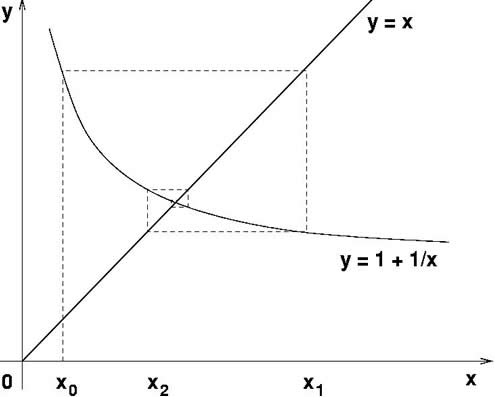
\includegraphics[width=0.3\textwidth]{./images/Spiral_Graph.jpg}
  \caption{Sequence of mappings must converge consider the graphs of $y=x$ and $y=1+1/x.$}
  \label{fig:spiral_graph}
  \end{figure}

The golden ratio is a mathematical wonder that transcends the boundaries between the conceptual and the practical. Its influence can be traced in the efficient inner workings of Fibonacci heaps, where it optimizes the data structure's performance and maintains its balance. The golden ratio also in the captivating spiral arrangement of leaves on plants, revealing a deep connection between mathematical order and biological growth. The ratio reveals itself and the power of mathematics to uncover the underlying principles that govern the world around us.

\begin{figure}[ht]
  \centering
  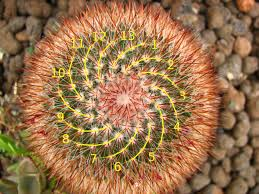
\includegraphics[width=0.3\textwidth]{./images/Cactus.png}
  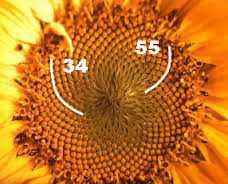
\includegraphics[width=0.3\textwidth]{./images/Sunflower.png}
  \caption{Fibonacci Numbers and Spiral Growth}
  \label{fig:cactus_spiral}
  \end{figure}

By virtue of allocating load according to the Fibonacci sequence, the FMLB protocol is in a sense algorithmically converging to the golden ratio as well. With more paths, the ratio of packets allocated to successive paths approaches the golden ratio. For instance, with 10 paths, the load allocation fractions are:
\[
\begin{aligned}
\frac{F_{10}}{143} : \frac{F_9}{143} : \frac{F_8}{143} : \frac{F_7}{143} : \frac{F_6}{143} &\approx 0.385 : 0.238 : 0.147 : 0.091 : 0.056, \\
\frac{F_5}{143} : \frac{F_4}{143} : \frac{F_3}{143} : \frac{F_2}{143} : \frac{F_1}{143} &\approx 0.035 : 0.021 : 0.014 : 0.007 : 0.007,
\end{aligned}
\]
The ratios of successive fractions are:
\[
1.618 : 1.619 : 1.615 : 1.625 : 1.6 : 1.667 : 1.5 : 2 : 1,
\]
which are all close to $\varphi \approx 1.618$.

So in a beautiful yet unexpected way, the FMLB protocol is harnessing the golden ratio, one of the most aesthetically pleasing mathematical constants, to achieve optimal load balancing and routing in complex networks. It's quite profound that a mathematical concept revered for its elegance but sometimes dismissed as impractical has found application in such a pertinent networking challenge. The appearance of the golden ratio here is also a reminder of the interconnectedness of different subfields of math and their occasional surprising practicality.


% Conclusion Section
The application of the Fibonacci sequence and golden ratio to the problem of load balancing in mobile ad hoc networks, as done by the FMLB protocol, exemplifies the beauty and power of mathematical ideas. It shows how abstract concepts, borne out of pure thought and aesthetic considerations, can inform very practical solutions. For mathematicians, it serves as an invitation to not only appreciate the theoretical elegance of objects like the Fibonacci numbers and golden ratio, but to also ponder their potential utility. Tashtoush et al.'s work demonstrates that mathematical beauty and practical application need not be distant ideas - they can come together in harmony to advance the frontiers of networking research. As we marvel at this seamless interplay of mathematical theory and real-world practice, we are reminded of the importance of both fundamental research and applied work. It is through their synergy that we uncover new insights and solve important problems - all while appreciating the mathematical beauty that underlies it all.



% Works Cited Page
\newpage
\begin{thebibliography}{9}

\bibitem{fmlbPaper} 
Yahya Tashtoush, Omar Darwish, Mohammad Hayajneh. 
"Fibonacci sequence based multipath load balancing approach for mobile ad hoc networks." 
\textit{Ad Hoc Networks}, Elsevier, 2014.

\bibitem{nrich}
"The Golden Ratio, Fibonacci Numbers and Continued Fractions." NRICH, 
\texttt{https://nrich.maths.org/2561}

\bibitem{mathIsFun}
"Nature, The Golden Ratio, and Fibonacci Numbers." Math Is Fun,
\texttt{https://www.mathsisfun.com/numbers/nature-golden-ratio-fibonacci.html}

\end{thebibliography}

\end{document}
